% Name: Cumulative distribution function
% Description: The standard normal CDF, with the 97.5th percentile at z = 1.96 traced to both axes.
% Tags: cumulative distribution, normal distribution, quantile, probability

\usepackage{pgfplots}
\pgfplotsset{compat=1.18}

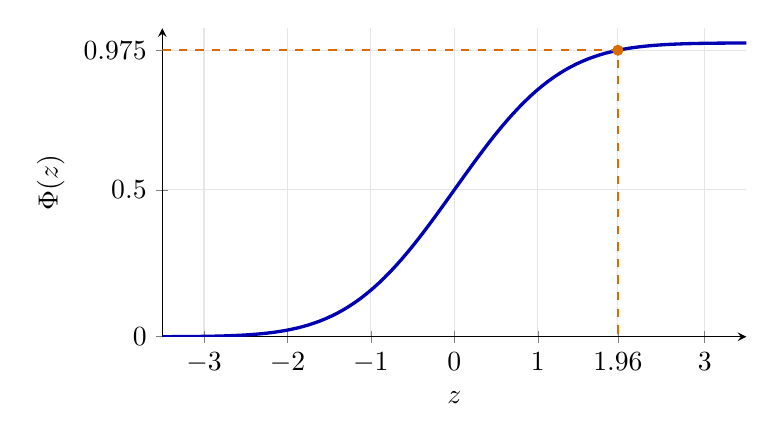
\begin{tikzpicture}
  \begin{axis}[
    width=9cm, height=5.5cm, domain=-3.5:3.5, samples=101,
    xmin=-3.5, xmax=3.5, ymin=0, ymax=1.05,
    axis lines=left, xlabel=$z$, ylabel={$\Phi(z)$},
    ytick={0,0.5,0.975}, yticklabels={$0$,$0.5$,$0.975$},
    xtick={-3,-2,-1,0,1,1.96,3}, xticklabels={$-3$,$-2$,$-1$,$0$,$1$,$1.96$,$3$},
    grid=major, grid style={gray!20},
    % Phi from the error function, with erf taken from Abramowitz and Stegun 7.1.26 (error below 1.5e-7).
    declare function={
      t(\x) = 1/(1 + 0.3275911*\x);
      erfp(\x) = 1 - t(\x)*(0.254829592 + t(\x)*(-0.284496736 + t(\x)*(1.421413741 + t(\x)*(-1.453152027 + 1.061405429*t(\x)))))*exp(-\x*\x);
      Phi(\z) = 0.5*(1 + sign(\z)*erfp(abs(\z)/sqrt(2)));
    },
  ]
    \addplot[very thick, blue!70!black] {Phi(x)};
    \draw[dashed, orange!85!black, thick] (axis cs:-3.5,0.975) -| (axis cs:1.96,0);
    \fill[orange!85!black] (axis cs:1.96,0.975) circle (2pt);
  \end{axis}
\end{tikzpicture}
